\section{ SR01MY22 }


\subsection{Meta}

    \textbf{Title:}
    AI for patient scheduling in the real-world health care setting: A metanarrative review

    \begin{table}[H]
        \centering
        \begin{tabular}{|c|c|c|c|c|c|c|c|c|}
            \hline
                \textbf{Rank} & \textbf{Grasp} & \textbf{Grade} & \textbf{Type} & \textbf{Outcome} & \textbf{Domain} & \textbf{COV19} & \textbf{CoI} & \textbf{DB} \\
            \hline
                5 & 90\% & B & A & P & S & No & - & No \\
            \hline
        \end{tabular}
        \caption{Reference's metadata}
        \label{tab:SR01MY22}
    \end{table}

\subsection{Summary}
    Mohamad Khairulamirin Md Razali et al. conducted a classical literature review analysing the critical parameters of the Master Scheduling Surgery Problem. The authors' biggest emphasis lies in the optimisation component of the MSSP solutions. The seven known databases were searched for studies from 2000 to 2021, prioritising the publications between 2016 and 2021. What stands out from the other literature reviews is that the analysis methods and benchmarking methods have been discussed. As well as other literature reviews, the identified research gap was found to need more implementations of the schedulers in real hospitals and a lack of actual medical records for research. An unexpected suggestion was given regarding the hyper-heuristic optimisation models. The authors stated that hyper-heuristics have been successful and widely used for other optimisation problems. Still, no studies highlight the utilisation of the hyper-heuristic scheduler for the MSSP. Overall, this literature review has three most valuable points: a list of databases for further study search, benchmark approaches, and a new view on the hyper-heuristic methods.
    

\subsection{Notes}
    \begin{itemize}
        \item Literature databases: Scopus, WoS, Dimensions.ai, SpringerLink, ACM Digital Library, IEEE Xplore, and Google Scholar;
        \item Has solution evaluation methods: Sensitivity Analysis, Robustness Analysis, Model Variation Analysis, Pareto Frontier Analysis, Simulation;
        \item Shortsights: ignoring objectives, priority of objectives, ignoring uncertainty, assumptions in hospital practice; 
        \item Challenges: Data Availability, Simulation vs Real World, Software Cost;
        \item What is hyper-heuristic?
    \end{itemize}


\subsection{Reading}
    \textbf{Abstract:}
    The Master Surgery Scheduling Problem (MSSP) assines the surgery cases to theatres, surgeons by specialty. In this literature review state-of-the-art MSSP problem have been analysed in studies from 2000 to 2021 focusing on the papers between 2016 and 2021. 
    
    \textbf{Objectives:}
    The work aims to overview the papers in the field of Master Surgery Scheduling Problem, identify trends and address the existing research gaps.

    
    \textbf{Page 1:}
    The MSSP represents one of the desicion levels descriped in (5). There is still some missalignments in terminology and only few studies addressed the MSSP in details.

    \textbf{Page 2:}
    Mohamad Khairulamirin Md Razali et al. enhpacise the difference between this and other literature reviews on MSSP by consentraiting on optimisation of MSSP. Then the questions of the research and methodology oitlined and the introduction to MSSP was presents.

    \textbf{Page 3:}
    This page continues to explain MSSP desicion-makng flow together with more details on the gathered studies (Focus January 1, 2016 - October 22, 2021).
    \begin{figure}[H]
        \centering
        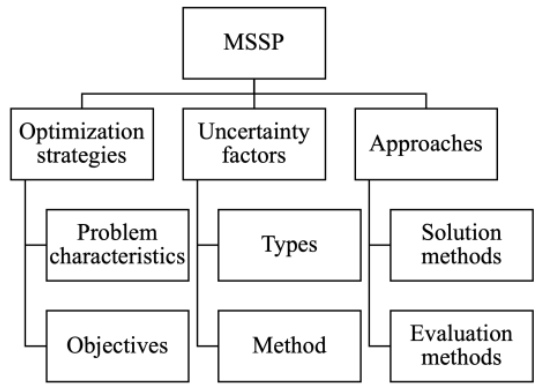
\includegraphics[width=.8\textwidth]{figures/0007_SR01MY22/fig1.png}
        \caption{MSSP classtering in \cite{x236}.}
        \label{fig1:0007_SR01MY22}
    \end{figure}

    \textbf{Page 4:}
    The authors describe the searching process and databases used. Then a simple comparative analysis was conducted on the several works. At the end of the page, types of the surgery group were introduced. 
    \begin{figure}[H]
        \centering
        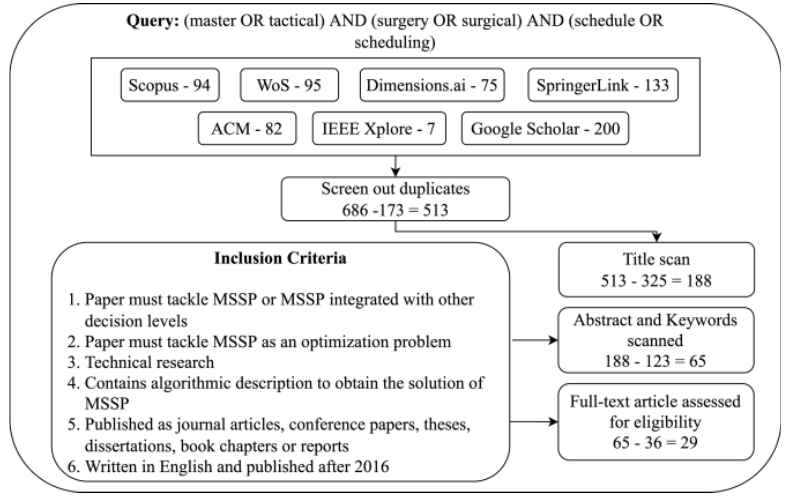
\includegraphics[width=.8\textwidth]{figures/0007_SR01MY22/fig2.png}
        \caption{Quantitative summary of the literature search in \cite{x236}.}
        \label{fig2:0007_SR01MY22}
    \end{figure}

    \textbf{Page 5:}
    The page consists of table with reference-contribution-applicability-limitation content of the overviewed studies.

    \textbf{Page 6:}
    Planning horizon and schedule cyclicity is described in general terms by referencing on the reviewed literature.
    \begin{figure}[H]
        \centering
        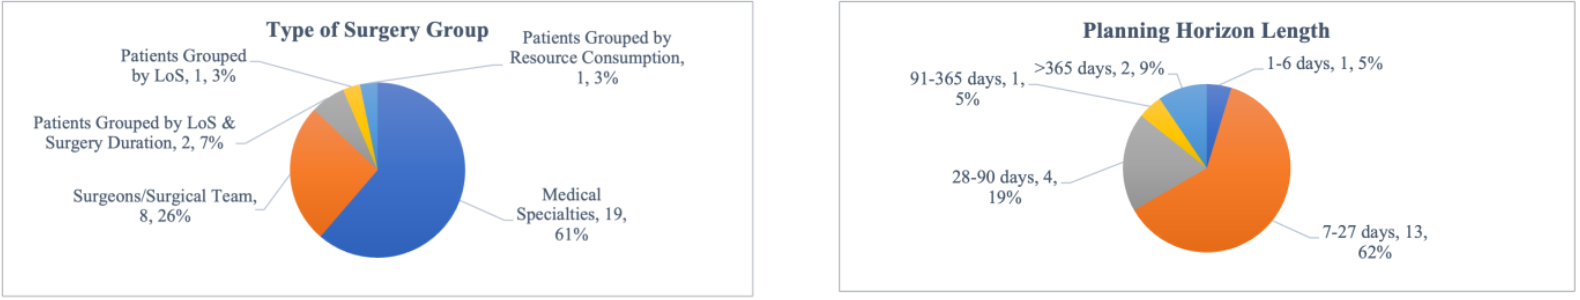
\includegraphics[width=.8\textwidth]{figures/0007_SR01MY22/fig3.png}
        \caption{Studies distribution by the surgery group type and by planning horizon in \cite{x236}.}
        \label{fig3:0007_SR01MY22}
    \end{figure}

    \textbf{Page 7:}
    The objectives and constraints are indicated in the literature and quantitative summary on the objective functions is shown below.
    \begin{figure}[H]
        \centering
        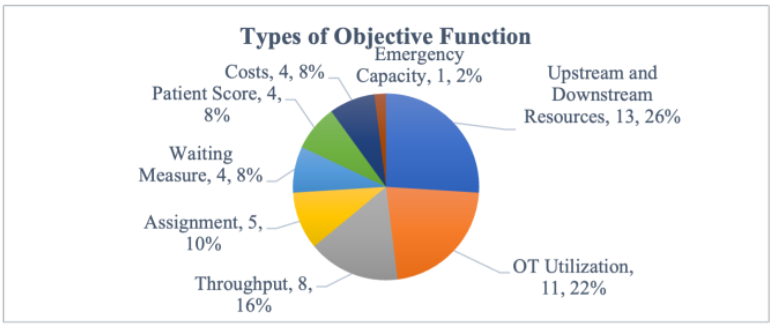
\includegraphics[width=.8\textwidth]{figures/0007_SR01MY22/fig4.png}
        \caption{Studies distribution by the objective functions in \cite{x236}.}
        \label{fig4:0007_SR01MY22}
    \end{figure}

    \textbf{Page 8:}
    In this page the disctibution of works with unsertainty and general overview of papers with different solution approaches (optimisation, heuristics).
    \begin{figure}[H]
        \centering
        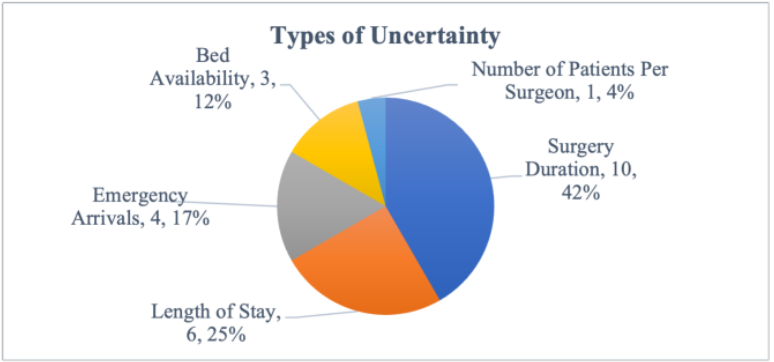
\includegraphics[width=.8\textwidth]{figures/0007_SR01MY22/fig5.png}
        \caption{Studies distribution by uncertainty in \cite{x236}.}
        \label{fig5:0007_SR01MY22}
    \end{figure}

    \textbf{Page 9:}
    The authors summarise the evaluation methods into distribution pie-chart and the table containing the reference, algorithm name, benchmark approach, and results.
    
    \textbf{Page 10:}
    Here the types of analyses used in the studies are presented as well at the obsticles or pure decissions made in the reviewed researches.
    
    \textbf{Page 11:}
    The authors highlight importance of the real hospital records as well as the practical implementation of the proposed solutions. The consern is rased that the financial resurces should also be spent optimaly for the MSSP solutions. In addition the suggestions regarding the scheduling cycles, uncertainty, computational complexity (hyper-heuristics), banchmarking.
    
    \textbf{Conclusion:}
    The authors repeat goals from the introduction to this research and hihglight the analysis of the papers from 2000 to 2021 in respect of uncertainty, used data, implementation, and solution approaches to MSSP. There are still uncharted territory in diration of stratefies for optimising efficiency, multiple decision levels, MSSP complexity, and aspects which influance objectices usage.